\section{Introduction}\label{sec:intro}

The goal of the OpenDreamKit project \cite{ODKproposal:on} is to develop a generic Toolkit
that will enable Mathematicians (and scientists in general) to build so-called Virtual
Research Environments (VREs) that are optimally tailored to specific communities. These
will combine a multitude of different tasks, such as symbolic mathematics, automatic code
generation, numerical computation, data bases, post-processing or visualisation. A VRE
will provide end-users with a single tool-chain that can be used for most, if not all, of
their research.

To be able to build such a toolkit, we will need to combine three different aspects of
``doing mathematics research'' -- Data (D), Knowledge (K) and Software (S). Ultimately we want to
create and make use of them using a VRE: we want to model the real world, translate it
into a set of mathematical objects and computationally simulate and thereby explore them.

Presently, the \emph{Data Aspect} is commonly implemented in special databases, such as
\LMFDB or \OEIS, that use tables or lists of numerical of symbolic data. The
\emph{Software Aspect} is represented by mathematical computation systems, such as \GAP,
\SageMath, and others that implement algorithms on top of this data. The \emph{Knowledge
  Aspect} is implemented in mathematical documents that describe mathematical concepts,
their meanings, and their properties.  The latter aspect includes at least the knowledge
underlying the data (e.g., the schemas of the database) and the software (e.g., the data
types involved in the computations) and thus bridges between those two. An illustration
with more examples of these aspects is given in Figure~\ref{fig:thebigpicture} (from the
\pn proposal).

\begin{figure}[ht]\centering
  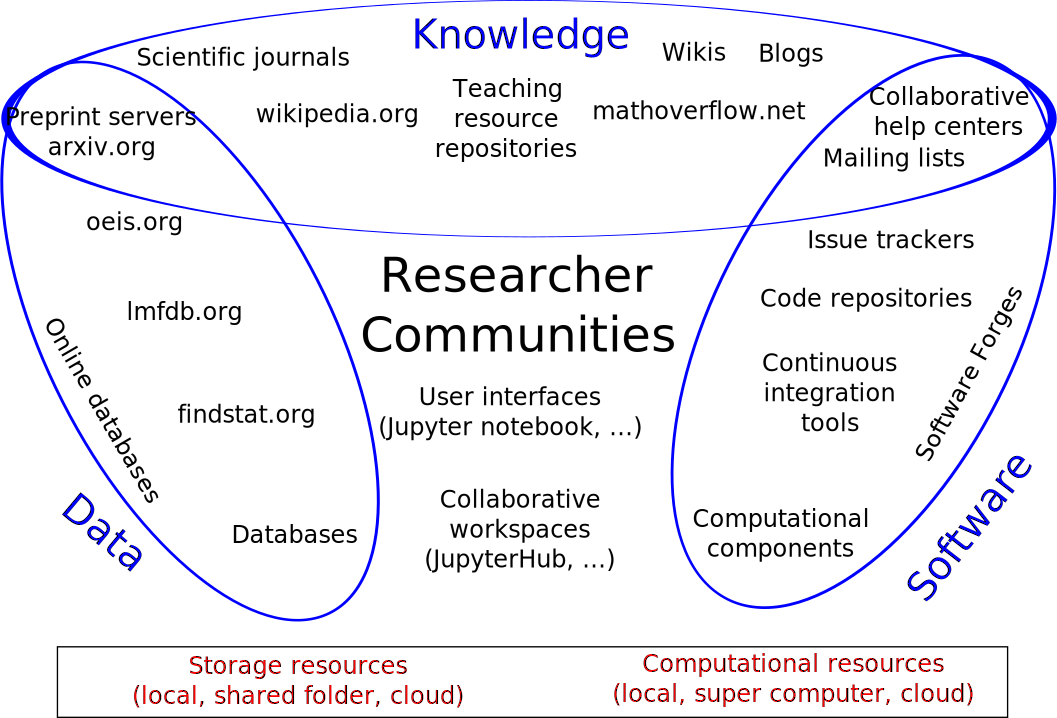
\includegraphics[width=\textwidth]{../../Proposal/Pictures/TheBigPicture.pdf}
  \caption{Virtual Research Environments for research in pure
    mathematics and applications.}
  \label{fig:thebigpicture}
\end{figure}

Notably, even though most systems combine elements from more than one aspect, each system has a clear primary aspect and uses only optional or auxiliary infrastructure for the other aspects.
For example, a computation system like \SageMath includes knowledge mostly in comments and data mostly in dedicated tables.
Similarly, database systems like \LMFDB includes a simple knowledge base for the relevant definitions and performs some mathematical computations in its frontend.
Thus, each system tends to be biased towards one aspect, and that makes interoperability between these systems unnecessarily difficult.

The approach of work package \WPtref{dksbases} in the \pn project is to model these three
aspects of mathematics research explicitly and uniformly.
This provides a strong theoretical basis for the envisioned mathematical
VRE toolkit. Concretely, the \pn proposal calls for an extension of the well-established
framework of theory graphs --- developed for the representation of mathematical knowledge
and languages (see Section~\ref{sec:MMT}) --- with Data and Software components to arrive
at a foundation for mathematical \DKS-bases. This deliverable report surveys
the results of the first year and presents the initial design for the
\DKS-bases.

In a series of workshops (September 2015 in Paris, January 2016 in St. Andrews, June 2016
in Bremen, and July 2016 in Bia{\l}ystok) the participants working on \WPref{dksbases} met
and discussed the topic of integrating the \pn systems into a mathematical VRE toolkit.
Key results were the observation that knowledge-aware interoperability of software and database-systems is critical
for \pn as well as the consensus that it can be achieved by aligning the mathematical knowledge underlying
the various systems.
This requires explicitly representing the three aspects of mathematical research and basing
computational services and inter-system communication on a joint \DKS-base.
These results are engrained in the ``Math-in-the-Middle'' (MitM)
paradigm~\cite{DehKohKon:iop16}, which is a central result of this report.

In the rest of this report, we describe the following:
\begin{compactenum}
\item In Section~\ref{sec:survey} we report on the initial survey of existing \pn-systems with
D/K/S aspects (see also Appendix~\ref{sec:raw-survey} for the raw data).
This survey was conducted at the Paris workshop in September 2015 as part of the \pn project.
Moreover, we derive requirements for a \DKS theory from that.
\item In Section~\ref{sec:MMT} we introduce the knowledge-driven OMDoc/\MMT framework, which we use as the
  starting point towards building DKS theories.
  This is a previously existing knowledge representation language.
  Because it already abstracts from system and language-specific idiosyncrasies, it is well-suited for providing the level of abstraction necessary for a system-integrating VRE.
  Our goal will be to extend it to the data and software aspects.
\item In Section~\ref{sec:mitm}, we present the MitM paradigm.
  This is a novel method that we have developed in \pn for integrating the \emph{software} systems into \emph{knowledge} representation.
\item In Section~\ref{sec:data}, we extend the \MMT language and system with novel explicit concepts for representing the data aspect.
\item In Section~\ref{sec:cases}, we present a few case studies of representing concrete software and data systems on top of our \DKS-bases.
\end{compactenum}

The resulting implementation of \DKS-bases on top of the \MMT system provides the basis for general VRE services, which can be developed in future \pn phases.
These include remote procedure call via the SCSCP protocol~\cite{SCSCP,FHKLR:SCSCP08,HorRoz:ossp09}, joint search engines over heterogeneous libraries of mathematical systems, or computational service discovery via MONET-like methods~\cite{aird-et-al:2005}.


%%% Local Variables:
%%% mode: latex
%%% TeX-master: "report"
%%% End:

%  LocalWords:  ODKproposal emph thebigpicture pn centering includegraphics textwidth
%  LocalWords:  WPtref dksbases mathcal ystok WPref realization DehKohKon iop16 nowledge
%  LocalWords:  impl RabKoh myxscale myyscale mitm compactenum formalizing KohManRab
%  LocalWords:  aumftg13 btc07 ossp09 aird-et-al
